\appendix

\chapter{Appendix: Geometry}\label{appendix}
This appendix investigates some facts and propositions pertaining to geometry in $\mathbb R^3$. Since marked points are not present here, the dashed notation introduced in Chapter \ref{ch:1} will be dropped.




\section{Calculating the circumdiameter}\label{A:CM}
\todoo[inline]{Check circumdiameter x circumradius, it's a bit confusing in many places}
Here we describe how to calculate the circumradius (or circumdiameter) of a $3$-simplex through the Cayley-Menger determinant (\cite{Cayley1841}, \cite{Menger28}, \cite{Uspensky48}). 

First, consider the points $p_1,\dots, p_5 \in \mathbb R^4$ which form a $4$-simplex. Denote $d_{ij} = \|p_i - p_j\|, i,j=1,\dots,5$. Then the area $A$ of the $4$-simplex is given by the \textbf{Cayley-Menger determinant} (\cite{Sommerville1929}). We have
\todoo[inline]{citation}. 

$$
-9216 A^2 =
\begin{vmatrix}
0 & 1 & 1 & 1 & 1 & 1 \\
1 & 0 & d^2_{12} & d^2_{13} & d^2_{14} & d^2_{15} \\
1 & d^2_{21} & 0 & d^2_{23} & d^2_{24} & d^2_{25}  \\
1 & d^2_{31} & d^2_{32} & 0 & d^2_{34} & d^2_{35} \\ 
1 & d^2_{41} & d^2_{42} & d^2_{43} & 0 & d^2_{45} \\
1 & d^2_{51} & d^2_{52} & d^2_{53} & d^2_{54} & 0 
\end{vmatrix}. 
$$
Now consider non-coplanar points $p_1,\dots, p_4 \in \Rt$ forming a $3$-simplex, i.e. a tetrahedron. To obtain the circumradius of this tetrahedron we imagine $p_1,\dots, p_4$ to lie on a $3$-dimensional hyperplane $H$ in $\mathbb R^4$ and we consider the point $c \in H$ such that $\|c-p_i\| = r$ for all $i=1,\dots,4$, $r\in \mathbb R$. The point $c$ is, by definition, the center of the circumsphere of $p_1,\dots,p_4$ and $r$ is the circumradius. The circumradius $r$ can be obtained using the Cayley-Menger determinant, since $p_1,\dots,p_4,c$ now form a $4$-dimensional simplex of volume $0$. We therefore have 


\begin{equation}\label{eq:CMeq}
0 = 
\begin{vmatrix}
0 & 1 & 1 & 1 & 1 & 1 \\
1 & 0 & d^2_{12} & d^2_{13} & d^2_{14} & r^2 \\
1 & d^2_{21} & 0 & d^2_{23} & d^2_{24} & r^2 \\
1 & d^2_{31} & d^2_{32} & 0 & d^2_{34} & r^2 \\ 
1 & d^2_{41} & d^2_{42} & d^2_{43} & 0 & r^2 \\
1 & r^2 & r^2 & r^2 & r^2 & 0 \\
\end{vmatrix}, 
\end{equation}
where we again have   $d_{ij} = \|p_i - p_j\|, i,j=1,\dots,4$.\newline  

It would be possible to solve \ref{eq:CMeq} as an equation of $r$. A better approach is to  subtract $r^2$ times the first row from the last row and subtract $r^2$ times the first column from the last column to obtain the determinant 



$$
\begin{vmatrix}
0 & 1 & 1 & 1 & 1 & 1 \\
1 & 0 & d^2_{12} & d^2_{13} & d^2_{14} & 0 \\
1 & d^2_{21} & 0 & d^2_{23} & d^2_{24} & 0 \\
1 & d^2_{31} & d^2_{32} & 0 & d^2_{34} & 0 \\ 
1 & d^2_{41} & d^2_{42} & d^2_{43} & 0 & 0 \\
1 & 0 & 0 & 0 & 0 & -2r^2 \\
\end{vmatrix}. 
$$
By expanding by the last row, we obtain the equation

$$
2r^2 \begin{vmatrix}
0 & 1 & 1 & 1 & 1 \\
1 & 0 & d^2_{12} & d^2_{13} & d^2_{14} \\
1 & d^2_{21} & 0 & d^2_{23} & d^2_{24} \\
1 & d^2_{31} & d^2_{32} & 0 & d^2_{34} \\ 
1 & d^2_{41} & d^2_{42} & d^2_{43} & 0 \\
\end{vmatrix} 
-
\begin{vmatrix}
1 & 1 & 1 & 1 & 1 \\
0 & d^2_{12} & d^2_{13} & d^2_{14} & 0 \\
d^2_{21} & 0 & d^2_{23} & d^2_{24} & 0 \\
d^2_{31} & d^2_{32} & 0 & d^2_{34} & 0 \\ 
d^2_{41} & d^2_{42} & d^2_{43} & 0 & 0 \\
\end{vmatrix} = 0,
$$
from which $r^2$ is directly expressible as

\begin{equation}\label{eq:Cayley-Menger-expanded}
r^2 
=
\frac{
\begin{vmatrix}
1 & 1 & 1 & 1 & 1 \\
0 & d^2_{12} & d^2_{13} & d^2_{14} & 0 \\
d^2_{21} & 0 & d^2_{23} & d^2_{24} & 0 \\
d^2_{31} & d^2_{32} & 0 & d^2_{34} & 0 \\ 
d^2_{41} & d^2_{42} & d^2_{43} & 0 & 0 \\
\end{vmatrix}}
{2 \begin{vmatrix}
0 & 1 & 1 & 1 & 1 \\
1 & 0 & d^2_{12} & d^2_{13} & d^2_{14} \\
1 & d^2_{21} & 0 & d^2_{23} & d^2_{24} \\
1 & d^2_{31} & d^2_{32} & 0 & d^2_{34} \\ 
1 & d^2_{41} & d^2_{42} & d^2_{43} & 0 \\
\end{vmatrix} 
}.
\end{equation}
It is worth noting that the determinant in the quotient cannot equal zero, since it is again a Cayley-Menger determinant and we assumed $p_1,\dots,p_4$ to be non-coplanar. 



\section{Bounding the circumdiameter}\label{sec:boundingdiameter}
This section derives the bounds used in Theorems \ref{thm:E1}, \ref{thm:E2}, \ref{thm:E3}, \ref{thm:E4}, and Propositions \ref{prop:maxcircum} and \ref{prop:maxPeta}. There, we considered the problem of bounding the circumdiameter of tetrahedra present in the tetrahedrization of a pseudo-periodic configuration $\x \in \bar\Gamma$. This problem can be seen finding the bound for the tetrahedra defined in Proposition \ref{prop:tetraInTess}  with ``perturbed'' points. We first state the problem in clear terms and then proceed to find the bound.

\subsection{Statement of the problem}
The problem of founding the bounds can be stated as the following two optimization problems. Recall the definition of $\rho$ and $a$ from Section \ref{sec:setA}. \newline

\noindent For the tetrahedron $T_1$, the problem is 
\begin{equation}\label{prob:tetra1}
\begin{aligned}
& \underset{p_1,p_2,p_3,p_4\in \Rt}{\text{maximize}}
& & \chi(\{p_1,p_2,p_3,p_4\}) \\
& \text{subject to}
& & \| p_i - t_i\| \leq \rho a, \quad t_i\in \Rt, i=1,2,3,4, \\
& & &\|t_i - t_j\| = a, \quad i=1,2,3,4. 
\end{aligned}
\end{equation}

\noindent To state the problem for the tetrahedron $T_2$, first denote 
$$D = \begin{pmatrix}
0 & \sqrt 2  a & a & a \\
\sqrt 2 a & 0 & a & a \\
a & a & 0 & a\\
a & a & a & 0
\end{pmatrix},
$$
and denote the entries of matrix $D$ as $d_{ij}, i,j=1,2,3,4$. Then the statement is:
\begin{equation}\label{prob:tetra2}
\begin{aligned}
& \underset{p_1,p_2,p_3,p_4\in \Rt}{\text{maximize}}
& & \chi(\{p_1,p_2,p_3,p_4\}) \\
& \text{subject to}
& & \|p_i - t_i\| \leq \rho a, \quad t_i\in \Rt, i=1,2,3,4, \\
& & & \|t_i-t_j\| = d_{ij}, \quad i,j=1,2,3,4.\\
\end{aligned}
\end{equation}
This is a non-linear optimization problem. We can arrive at its solution through some careful geometric arguments.

\PlaceText{0.01cm}{29.3cm}{\tiny{?\v{s}}}
\subsection{Solution to the problem}
First, define the \textit{circumdiameter function} of point $p \in \Rt$ with respect to non-collinear points $p_1,p_2,p_3 \in \Rt$:
$$c(p) = \chi(\{p,p_1,p_2,p_3\}).$$
Denote $(x_i,y_i,z_i)$ the coordinates of $p_i, i=1,\dots,3$. Denote $\chi(\{p_1,p_2,p_3\})$ the circumdiameter of the triangle formed by $p_1,p_2,p_3$. Lastly, we remind the reader that a closed halfspace is a set of the form $\{y\in \Rt: \langle y, x \rangle \geq a\}, x\in\Rt, a\in \R $, and a open halfspace has the same form with a strict inequality.

The following lemma describes the properties of $c(p)$.

\begin{lemma} $c(p)$ is continuous, has a global minimum $c_{min} := \chi(\{p_1,p_2,p_3\})$ and level sets 
	$$L_a := \{p \in \Rt: c(p)=a\} = S_{a1} \cup S_{a2}, \quad a \geq c_{min},$$ 
	where $S_{a1}$ and $S_{a2}$ are two spheres with diameter $a$ such that $p_1,p_2,p_3 \in S_{a1}\cap S_{a2}$. Furthermore, the centers $c_1, c_2$ of $S_{a1},S_{a2}$ respectively, lie in the closed halfspaces
$$H_+ = \{x \in \Rt: Ax \geq 0 \},\; H_- = \{x \in \Rt: Ax \leq 0\},$$
respectivelly, where $A$ defines the hyperplane $H=\{x\in\Rt: Ax = 0\}$ such that $p_1,p_2,p_3\in H$. 
\end{lemma}
\begin{proof}
	Continuity: From \ref{eq:Cayley-Menger-expanded} we see that $c(p)$ can be seen as a composition of a norm, determinants and division. Determinant is continuous as a function of elements of the matrix since it is a polynomial function. Thus $c(p)$ is continuous.\newline

\noindent We can rewrite $L_a$ as
$$\{p \in \Rt: \exists \text{ sphere } S \text{ s.t. } p_1,p_2,p_3,p \in S \text{ and diam}S = a\}.$$
We must therefore find the number of spheres through the points $p_1,p_2,p_3$ with the diameter $a$. Denote $S$ a sphere such that $\{p_1,p_2,p_3\}\subset S$ with \mbox{$\mathrm{diam}(S)=a$}. Define the hyperplanes
$$H_{12} = \{x\in\Rt: \|x-p_1\| = \|x-p_2\|\}, \;\; H_{23} = \{x\in\Rt: \|x-p_2\|=\|x-p_3\|\}.$$
The intersection $H_{12}\cap H_{23}$ is a line $L$, as $p_1,p_2,p_3$ are non-collinear.  The center of $S$ is at distance $a/2$ from all three points and thus lies on $L$. For any point, there are at most two points on the line $L$ at a given distance from the point. This proves that there are at most two spheres satisfying the definition of $S$.

The point on $L$ at a minimum distance to $p_1,p_2,p_3$ is the point $p_{min}:=L\cap H$. We know that $p_{min}$ is equidistant from $p_1,p_2,p_3$ and that it lies on the hyperplane $H$, therefore it is the circumcenter of the triangle defined by $p_1,p_2,p_3$ and we have $c(p_{min}) = \chi(\{p_1,p_2,p_3\})$.  

\todoo[inline]{Could probably be simpler, but don't have time.}
To see that $c_1$ and $c_2$ must be (non-strictly) separated by the hyperplane $H$, assume, without loss of generality, that $\{c_1,c_2\}\subset H_+, c_1\neq c_2$. Let $p \in S_{a1}\setminus H$ and let  \mbox{$p_H\in \Rt$} be the reflection of $p$ through the hyperplane $H$. The tetrahedron $p_1,p_2,p_3,p_H$ then is a reflection of the tetrahedron $p_1,p_2,p_3, p$ and therefore its circumsphere has diameter $a$. However, its centre lies in $H_-$, which is a contradiction. 
\end{proof}

Note that $S_{a1}$ and $S_{a2}$ are not necessarily distinct. In fact, we can see from the proof that $S_{a1}=S_{a2}$ precisely when $a=c_{min}$.


We are now ready to characterize the set of solutions to \ref{prob:tetra1} and \ref{prob:tetra2}. For the next proposition, we say a point lies ``inside'' or ``outside'' of the sphere $S$ if the point lies in $B$ or in $B^c$ respectively, where $B$ is the closed ball such that $\partial B = S$. Further define $S(q_1,q_2,q_3,q_4)$ to be the sphere on which $q_1,q_2,q_3,q_4\in\Rt$ lie. We further define \textit{tangent spheres} as two spheres intersecting at a point. If one sphere lies inside the other, they are \textit{internally tangent}, otherwise they are \textit{externally tangent}. 


\begin{proposition}\label{prop:ApolloniusSet}
Any solution $(p_1,p_2,p_3,p_4)$ of the problem \ref{prob:tetra1} will lie on a sphere $S$ that is (internally or externally) tangent to the spheres $\partial B(t_i,\rho a), i =1,2,3,4$. 
\end{proposition}
\begin{proof}
	Let $(p_1,p_2,p_3,p_4)$ be a solution of \ref{prob:tetra1}. Denote $c(p)=\chi(\{p,p_2,p_3,p_4\})$, $ p \in \Rt$ and $S$ the circumsphere of $\{p_1,\dots,p_4\}$. 
	First assume that $p_1 \in B(t_1,\rho a)$. Because $p_1$ maximizes the function $c(p)$, we have $c(p_1)\geq c(p), p\in U$, where $U$ is some small neighborhood of $p_1$. Choose two points, $p_O,p_I\in U\setminus S$ such that 
\begin{enumerate} 
\item $c(p_O)=c(p_I)=b$,
\item $p_I$ is on the inside of $S$ and $p_0$ on the outside of $S$,
\item $S(p_I,p_2,p_3,p_4)$ and $S(p_O,p_2,p_3,p_4)$ do not equal and their centers lie on the same open halfspace (with respect to the hyperplane defined by $p_2,p_3,p_4$) as $S$. 
\end{enumerate}
Such choice is possible due to continuity of $c(p)$. Yet we arrive at a contradiction, as the level set $L_b$ now contains two distinct spheres with centres in the same open halfspace. 

Assume now that $p_1 \in \partial B(t_1,\rho a)$ and denote $S_1=\partial B(t_1,\rho a)$. We now choose $p_I$ and $p_O$ with the additional requirement that they must both lie on $\partial B(t_1,\rho a)$. Such choice is not possible precisely when $S_1$ and $S$ are tangent, since then  $S_1$ lies either completely inside or outside $S$ and it is no longer possible to choose points both outside and inside. 
\end{proof}
\unsure{Is this a good way of proceeding?}Note that Proposition \ref{prop:ApolloniusSet} is formulated for problem \ref{prob:tetra1}. However, we could repeat the same exact argument for \ref{prob:tetra2} and thus the same holds for both problems.\newline

We have found that the solutions to \ref{prob:tetra1} and \ref{prob:tetra2} must lie on a sphere that is tangent to the spheres within which points can move. This is a dramatic improvement --- we have narrowed the previously infinite space of possible solutions down to just $2^4=16$ possible quadruples of points (and even fewer because of symmetries). We also note that the set of solutions to our problem is precisely the set of solutions of a three-dimensional equivalent of the more than two thousand years old \textbf{Apollonius problem} (\cite{GischRibando2006}).


\subsection{Apollonius problem in $\mathbb R^3$}
We want to find all the spheres that are externally or internally tangent to the spheres $\partial B(t_i,\rho a), i=1,2,3,4$ as defined in problems \ref{prob:tetra1} and \ref{prob:tetra2}.

First note that two externally tangent spheres $S_1=((x_1,y_1,z_1),r_1)$, $S_2=((x_2,y_2,z_2),r_2)$  satisfy
$$\|(x_1,y_1,z_1) - (x_2,y_2,z_2)\| = r_1+r_2.$$
Similarly, two internally tangent spheres satisfy
$$\|(x_1,y_1,z_1) - (x_2,y_2,z_2)\| = |r_1 - r_2|.$$
By squaring both equations, we obtain the equality
$$(x_1-x_2)^2 + (y_1-y_2)^2 + (z_1-z_2)^2 = (r_1 \pm r_2)^2$$
Where we use $+$ for externally and $-$ for internally tangent spheres.

The Apollonius problem for spheres $S_1,S_2,S_3,S_4$ is therefore solved by any $S=((x,y,z),r)$ such that
\begin{align}\label{eq:Apollonius}
  (x_1-x)^2 + (y_1-y)^2 + (z_1-z)^2 &= (r_1 \pm r)^2 \\
  (x_2-x)^2 + (y_2-y)^2 + (z_2-z)^2 &= (r_2 \pm r)^2 \nonumber \\
  (x_3-x)^2 + (y_3-y)^2 + (z_3-z)^2 &= (r_3 \pm r)^2 \nonumber \\
  (x_4-x)^2 + (y_4-y)^2 + (z_4-z)^2 &= (r_4 \pm r)^2, \nonumber  
\end{align}

where we can take any combination of $+$ or $-$, yielding altogether $16$ possible solutions. We do not consider degenerate cases as they cannot happen in our setting. 

As noted previously, the number of solutions for both $T_1$ and $T_2$ will reduce significantly. For $T_1$, the spheres are completely interchangeable and thus only solutions with different number of $+$ will differ. This yields $5$ possible solutions. Geometrically the number of $+$ can be seen as the number of spheres the solution is externally tangent to. For $T_2$ the situation is more complex, as the problem is not entirely symmetric with respect to the four points. Still, symmetries do exist and the number of solution will be reduced.  

Sadly, for most choices of $+$ and $-$, these equations still seem to be too complex for Mathematica to solve. Luckily, we can simplify them further. 

\subsubsection{Solving the equations \eqref{eq:Apollonius} by linearizing}

We formulate the solution as a theorem.
\begin{theorem}\label{thm:Apollonius}
	For $\rho < 1/(2\sqrt 6)$, the maximum in \ref{prob:tetra1} is $a \chi_1$, where
	$$\chi_1 := 2(\sqrt 6/4 + \rho).$$
	For $\rho < 1/4$, the maximum in \ref{prob:tetra2} is $a \chi_2$, where
	$$\chi_2 := 2 \frac{2\rho + \sqrt{2 - 32\rho^2 + 64 \rho^4}}{2-32\rho^2}.$$

\end{theorem}
\begin{proof}
	Recall that the solution must lie on a sphere solving the equations \eqref{eq:Apollonius}. We must therefore solve them and find the solution with the largest circumdiameter.

First, for clarity, we define the variables $s_i\in\{+1,-1\},i=1,\dots,4$ instead of relying on the notation $\pm$. We begin by expanding the parentheses to obtain the equations
$$x^2+y^2+z^2 + x_i^2 + y_i^2 + z_i^2 - 2xx_i - 2yy_i - 2zz_i = r^2 + r_i^2 + 2s_i r_i r,\quad i=1,2,3,4$$

By subtracting the second, third, and fourth equation from the first, we get rid of the quadratic terms and obtain a system of linear equations with four variables and three equations:
\begin{align*}-&2(x_1-x_i)x - 2(y_1-y_i)y -2 (z_1-z_i)z - 2(s_1r_1 - s_2r_2)r \\
	& + x_1^2-x_i^2 + y_1^2-y_i^2 + z_1^2 - z_i^2 -r_1^2 + r_i^2 = 0, \quad i=2,3,4
\end{align*}
This system can be solved to obtain expression of $x,y,z$ in terms of $r$. We then substitute those expression into \eqref{eq:Apollonius} to obtain $r$\footnote{Note that exact solutions of $x,y,z$, which we are not interested in, could then by obtained through substituting $r$ back into the linear system.}. 

We have used Wolfram Mathematica (\cite{Mathematica}) to find the solutions. The full implementation can be found in the file \texttt{ApolloniusProblem.nb}. By comparing the circumdiameters of the solutions, we obtain the proposition.

\end{proof}
All the solutions for the choice $a=1$ can be seen in Figures \ref{fig:Apollonius1} and \ref{fig:Apollonius2}. We can see that for $T_1, \rho < 1/\sqrt 6$, we have the two solutions
$$a(\sqrt 6 / 4 + \rho), a \frac{\rho - \sqrt 6 (4\rho^2 - 1)}{4-24 \rho^2}$$
which intersect at $\rho =1/(2\sqrt 6)$. 

Notice the simple linear form of the first solution --- it is precisely the sphere which is internally tangent to all four spheres. This sphere has the same center as the circumsphere of tetrahedron $\{t_1,t_2,t_3,t_4\}$. Thus the solution is a sum of circumradius of the tetrahedron, $a \sqrt 6 /4$, and the radius of the four spheres, $\rho$. We can see similar behaviour in the solution that is externally tangent to all four spheres.

For $T_2$, the linear solution will no longer be the largest, as now we obtain a larger circumradius by using a sphere that is externally tangent to some of the spheres. 


\begin{remark}[General position]\label{rem:GP}
	From the form of the solutions one can also obtain the necessary bounds for $\rho$ for the points to remain in general position. The points cease to be in general position precisely when any one of the solutions becomes infinite. This gives us $\rho < 1/(2\sqrt 6)$ for $T_1$ and $\rho<1/4$ for $T_2$. Since we must control the circumdiameter for all tetrahedra, we must assume $\rho < 1/4$.
\end{remark}


\begin{figure}
	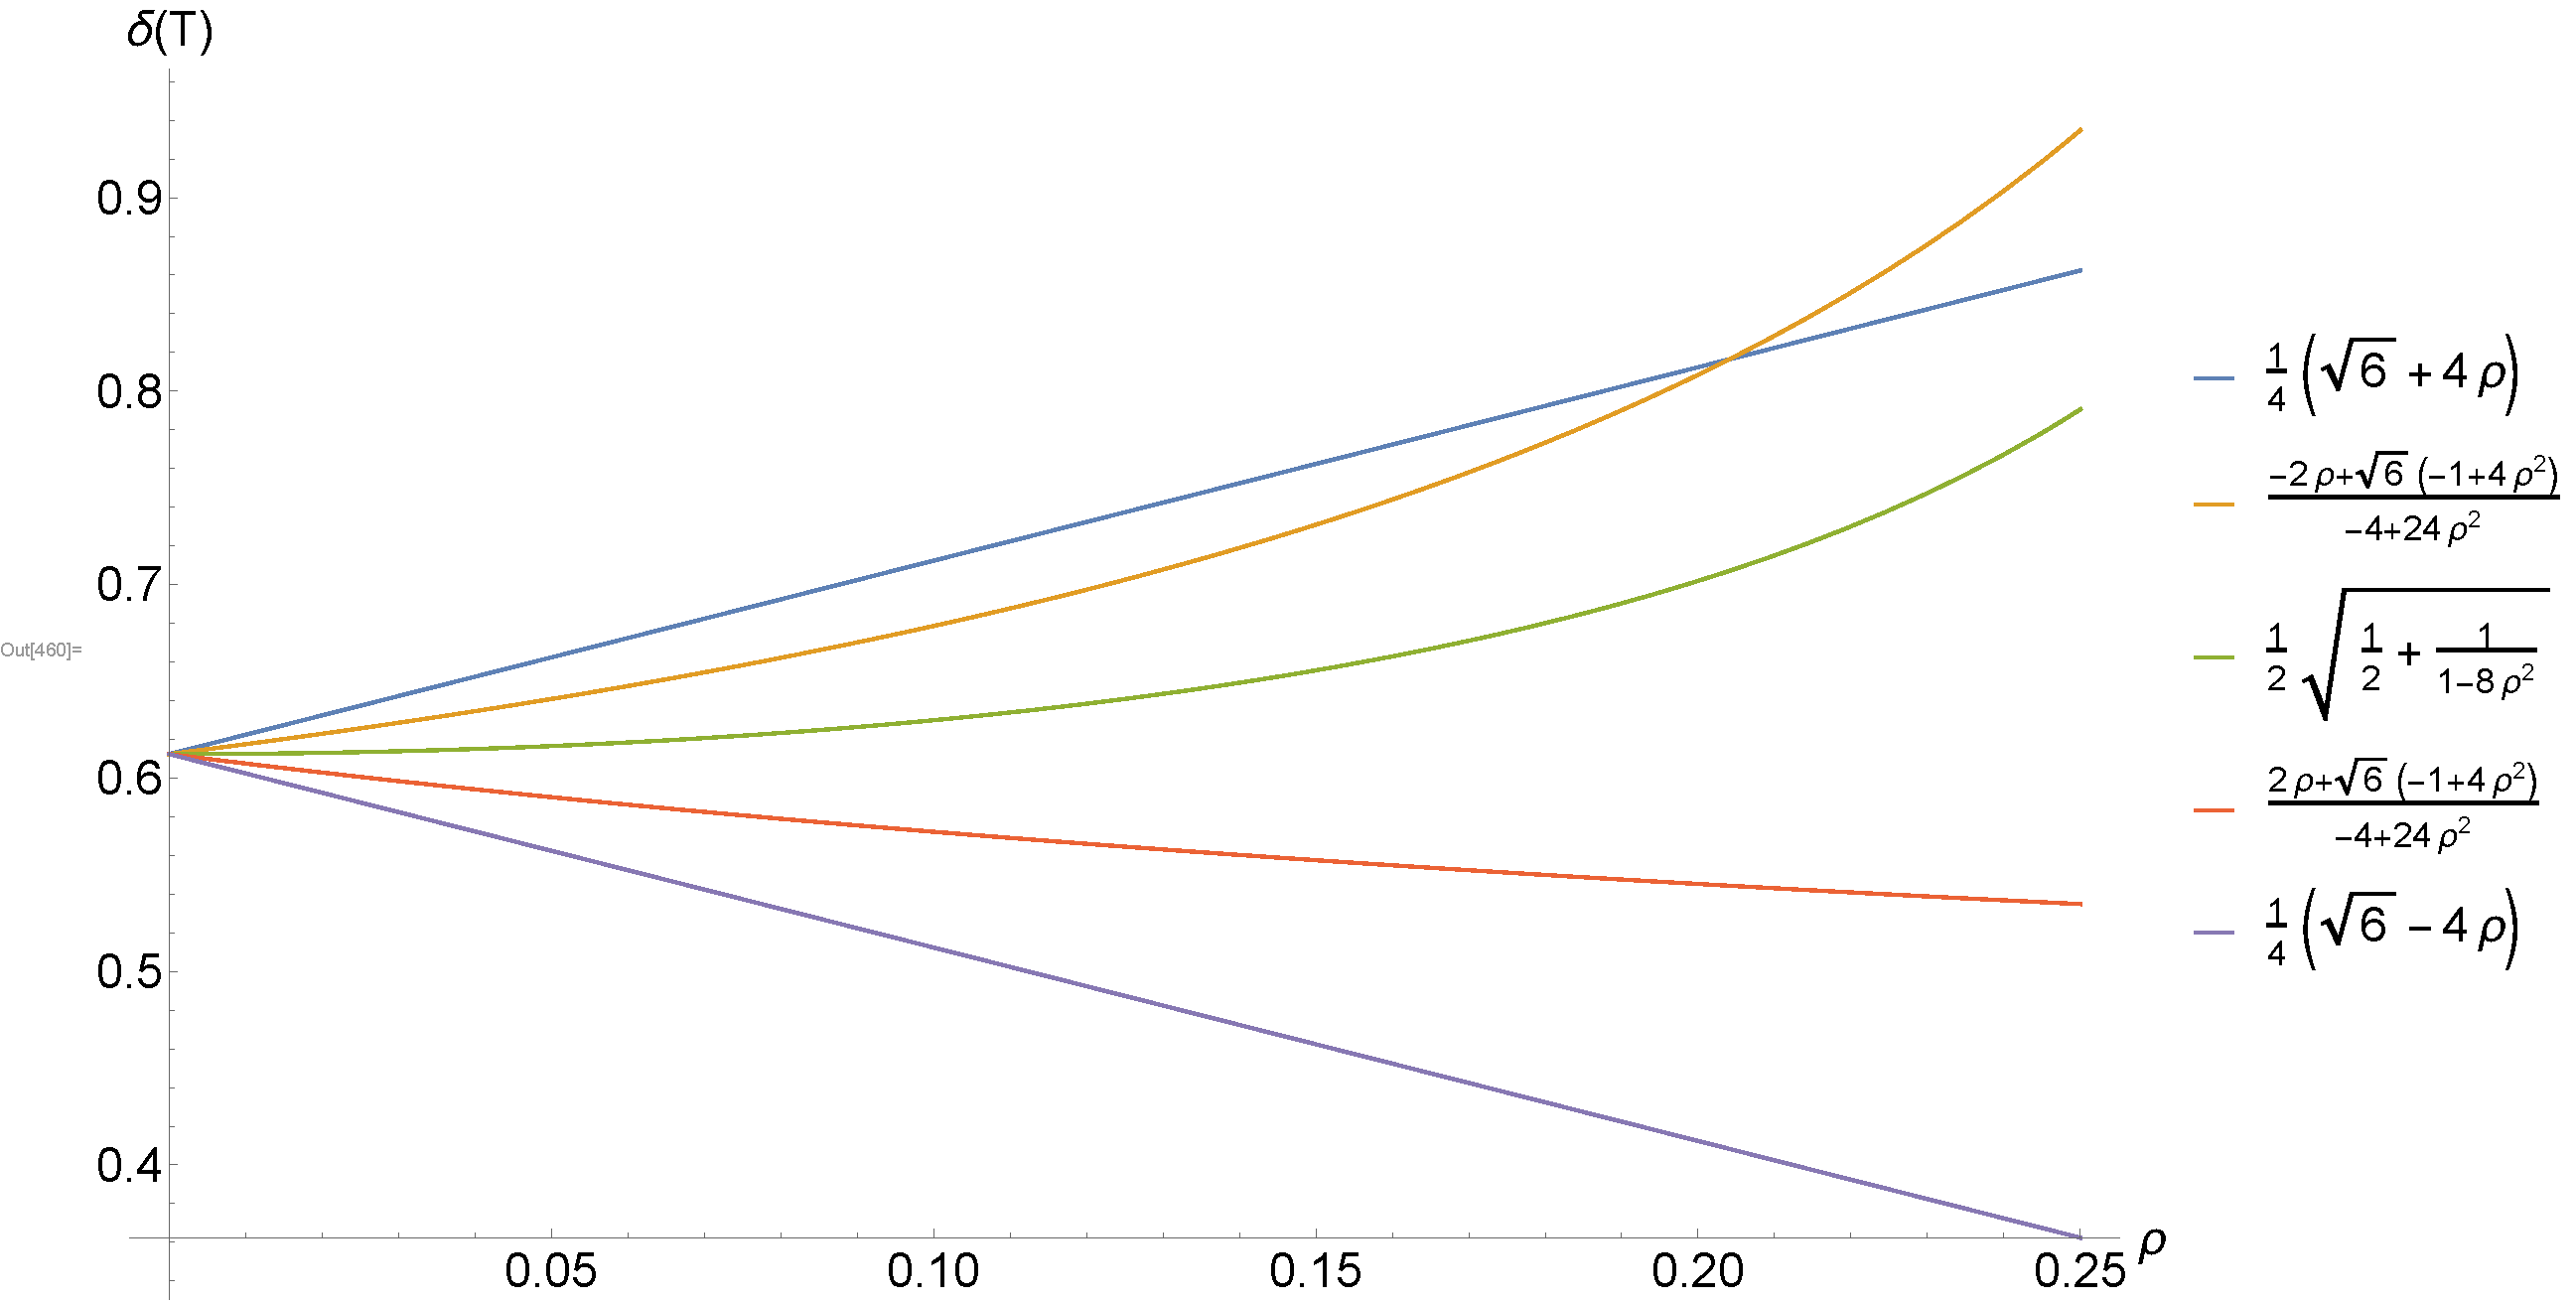
\includegraphics[width=1\textwidth]{../img/t1.pdf}
	\caption{All solutions to Apollonius problem with $T_1$, $a=1$.}\label{fig:Apollonius1}
\end{figure}

\begin{figure}
	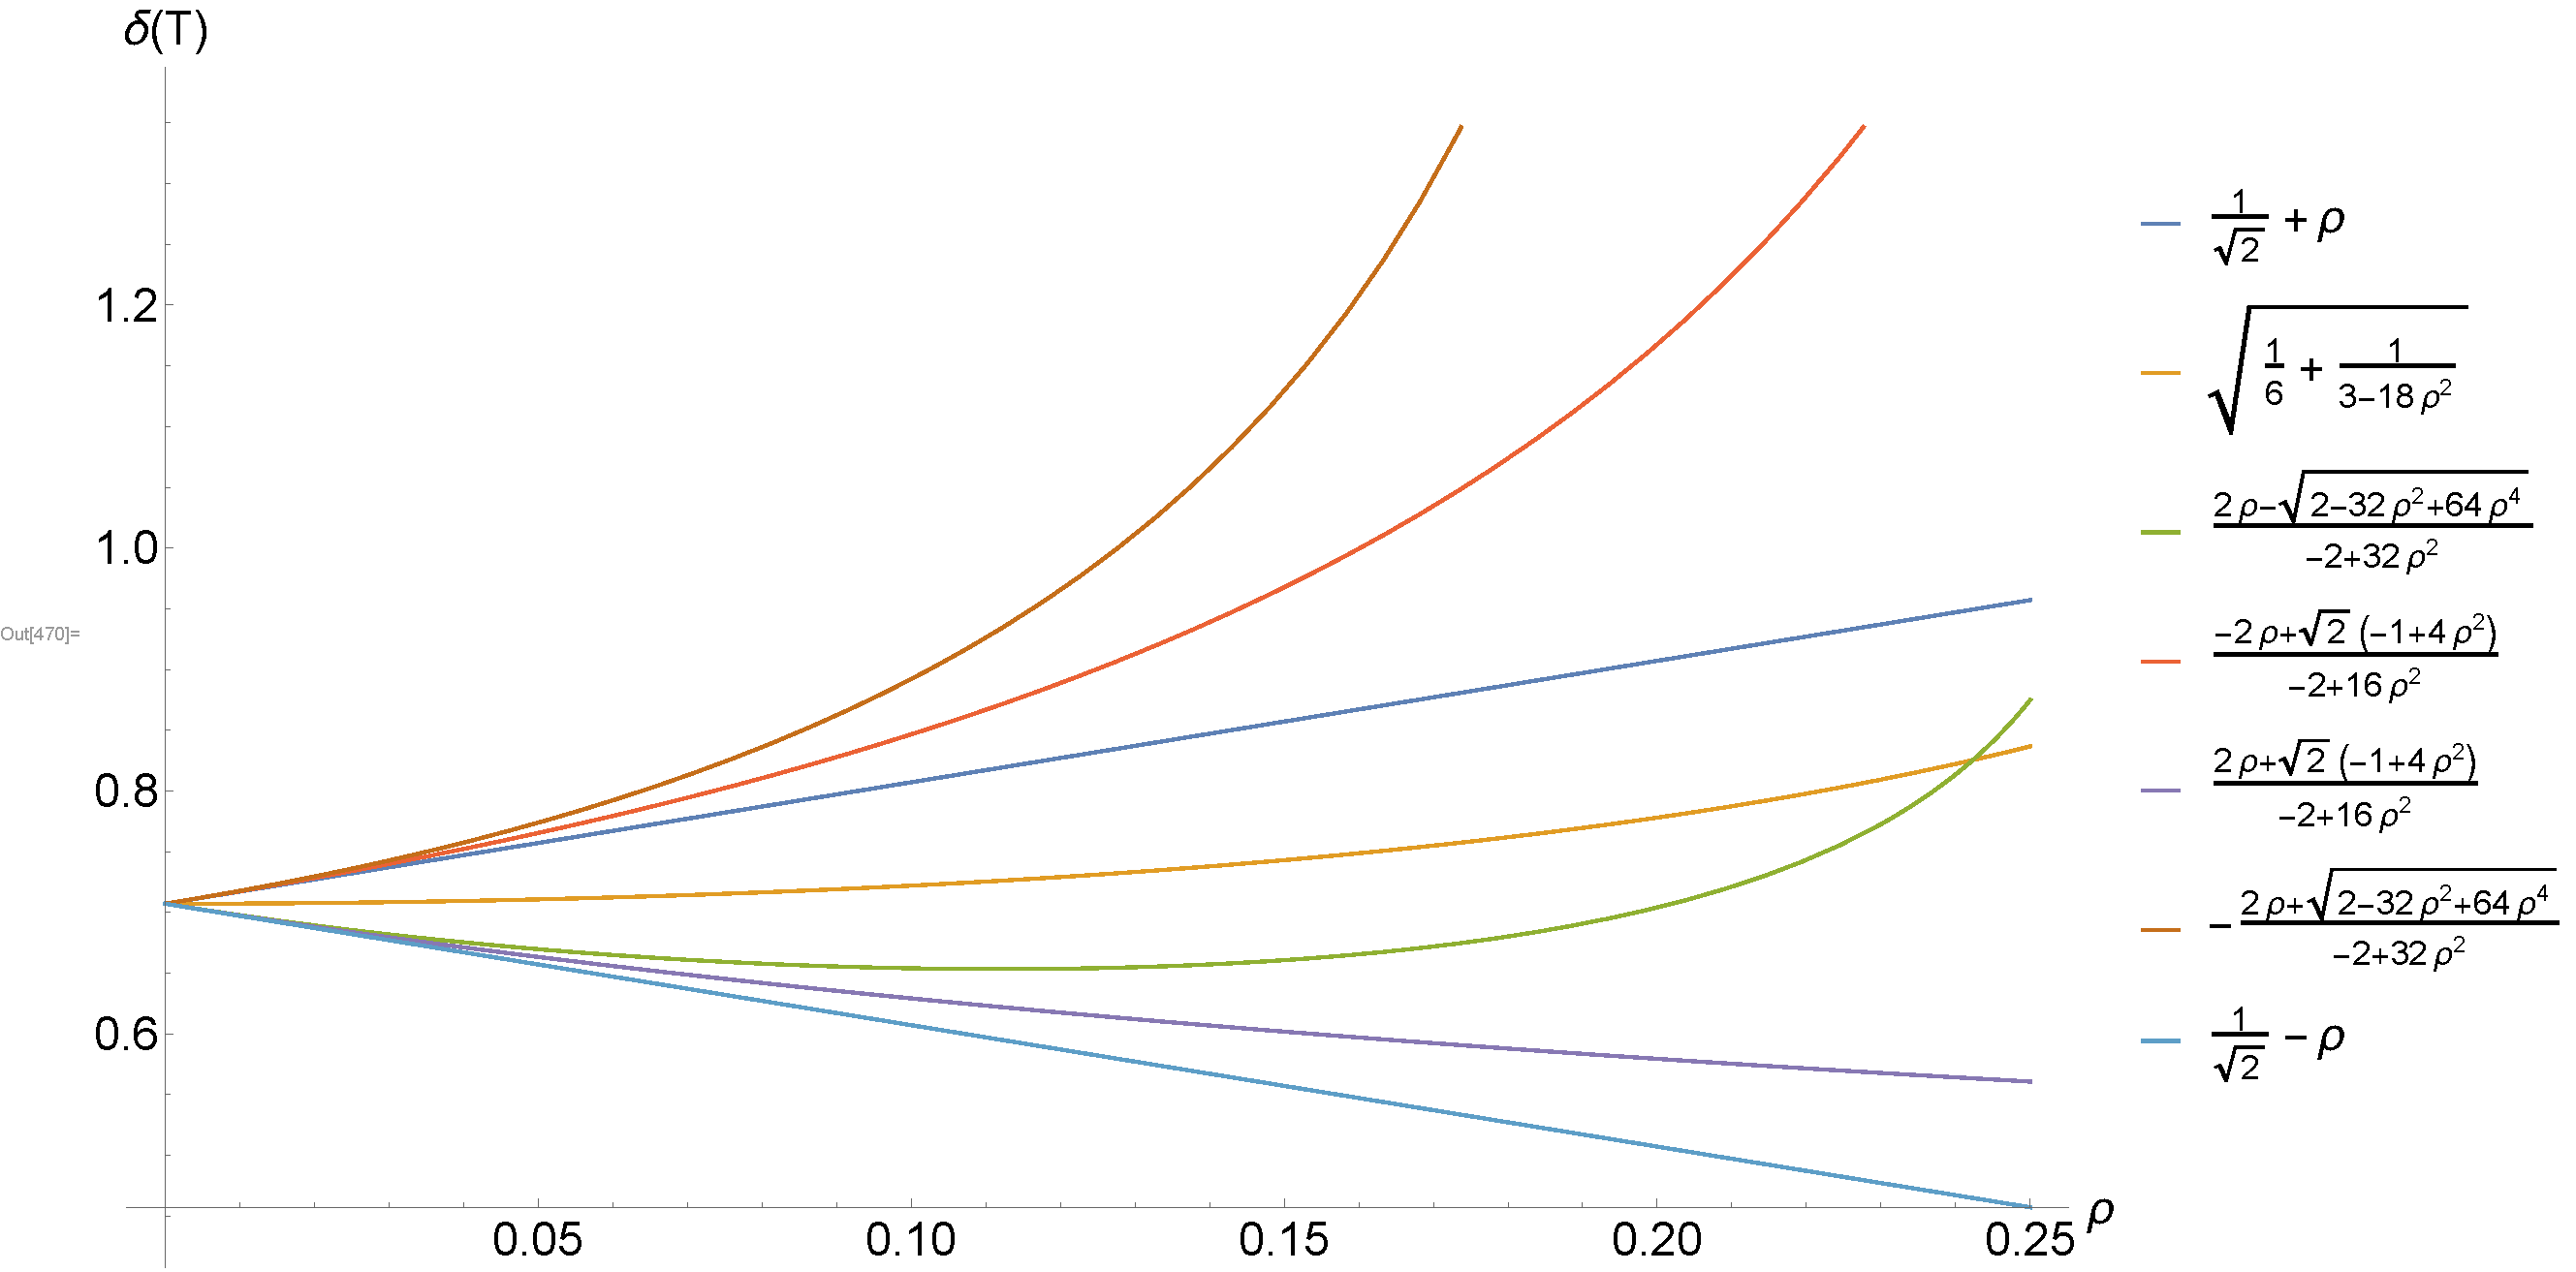
\includegraphics[width=1\textwidth]{../img/t2.pdf}
	\caption{All solutions to Apollonius problem with $T_2$, $a=1$}\label{fig:Apollonius2}
\end{figure}
